%% abtex2-modelo-trabalho-academico.tex, v-1.9.1 laurocesar
%% Copyright 2012-2013 by abnTeX2 group at http://abntex2.googlecode.com/ 
%%
%% This work may be distributed and/or modified under the
%% conditions of the LaTeX Project Public License, either version 1.3
%% of this license or (at your option) any later version.
%% The latest version of this license is in
%%   http://www.latex-project.org/lppl.txt
%% and version 1.3 or later is part of all distributions of LaTeX
%% version 2005/12/01 or later.
%%
%% This work has the LPPL maintenance status `maintained'.
%% 
%% The Current Maintainer of this work is the abnTeX2 team, led
%% by Lauro César Araujo. Further information are available on 
%% http://abntex2.googlecode.com/
%%
%% This work consists of the files abntex2-modelo-trabalho-academico.tex,
%% abntex2-modelo-include-comandos and abntex2-modelo-references.bib
%%

% ------------------------------------------------------------------------
% ------------------------------------------------------------------------
% abnTeXf2: Modelo de Trabalho Academico (tese de doutorado, dissertacao de
% mestrado e trabalhos monograficos em geral) em conformidade com 
% ABNT NBR 14724:2011: Informacao e documentacao - Trabalhos academicos -
% Apresentacao
% ------------------------------------------------------------------------
% ------------------------------------------------------------------------

\documentclass[
	% -- opções da classe memoir --
	12pt,				% tamanho da fonte
	openany,			% capítulos começam em qualquer página (para iniciar em página ímpar, tente openright)
	twoside,			% para impressão em páginas corretamente
	a4paper,			% tamanho do papel. 
	% -- opções da classe abntex2 --
	%chapter=TITLE,		% títulos de capítulos convertidos em letras maiúsculas
	%section=TITLE,		% títulos de seções convertidos em letras maiúsculas
	%subsection=TITLE,	% títulos de subseções convertidos em letras maiúsculas
	%subsubsection=TITLE,% títulos de subsubseções convertidos em letras maiúsculas
	% -- opções do pacote babel --
	english,			% idioma adicional para hifenização
	french,				% idioma adicional para hifenização
	spanish,			% idioma adicional para hifenização
	brazil,				% o último idioma é o principal do documento
	oldfontcommands
	]{abntex2}

% ---
% Pacotes básicos 
% ---
\usepackage{lmodern}			% Usa a fonte Latin Modern			
\usepackage[T1]{fontenc}		% Selecao de codigos de fonte.
\usepackage[utf8]{inputenc}		% Codificacao do documento (conversão automática dos acentos)
\usepackage{lastpage}			% Usado pela Ficha catalográfica
\usepackage{indentfirst}		% Indenta o primeiro parágrafo de cada seção.
\usepackage{color}				% Controle das cores
\usepackage{graphicx}			% Inclusão de gráficos
\usepackage{microtype} 			% Melhorias de justificação
\usepackage{pdfpages}			% Inserir páginas de pdf
% ---
		
% ---
% Pacotes adicionais, usados apenas no âmbito do Modelo Canônico do abnteX2
% ---
\usepackage{lipsum}				% para geração de dummy text
% ---

% ---
% Pacotes de citações
% ---
\usepackage[brazilian,hyperpageref]{backref}
% Paginas com as citações na bibl
\usepackage[num]{abntex2cite}	% Citações padrão ABNT

% --- 
% CONFIGURAÇÕES DE PACOTES
% --- 

% ---
% Configurações do pacote backref
% Usado sem a opção hyperpageref de backref
\renewcommand{\backrefpagesname}{Citado na(s) página(s):~}
% Texto padrão antes do número das páginas
\renewcommand{\backref}{}
% Define os textos da citação
\renewcommand*{\backrefalt}[4]{
	\ifcase #1 %
		Nenhuma citação no texto.%
	\or
		Citado na página #2.%
	\else
		Citado #1 vezes nas páginas #2.%
	\fi}%
% ---

% ---
% Informações de dados para CAPA e FOLHA DE ROSTO
% ---
\titulo{Sistema de controle de atitude para satélite CubeSat}
\autor{Augusto Bonangelo Costa\\
Felipe Ramos de Faria\\
William Mazi}
\local{São Caetano do Sul}
\data{2015}
\orientador{Prof. Dr. Rodrigo Alvite Romano}
%\coorientador{Professor}
\instituicao{Escola de Engenharia Mauá do Centro Universitário do Instituto Mauá de Tecnologia}
\tipotrabalho{Trabalho de Conclusão de Curso de Engenharia de Controle e Automação}
% O preambulo deve conter o tipo do trabalho, o objetivo, 
% o nome da instituição e a área de concentração 
\preambulo{Trabalho de Conclusão de Curso apresentado à Escola de Engenharia Mauá do Centro Universitário do Instituto Mauá de Tecnologia como requisito parcial para a obtenção do título de Engenheiro de Controle e Automação.}
% ---

% ---
% Configurações de aparência do PDF final

% alterando o aspecto da cor azul
\definecolor{blue}{RGB}{41,5,195}

% informações do PDF
\makeatletter
\hypersetup{
     	%pagebackref=true,
		pdftitle={\@title}, 
		pdfauthor={\@author},
    	pdfsubject={\imprimirpreambulo},
	    pdfcreator={LaTeX with abnTeX2},
		pdfkeywords={abnt}{latex}{abntex}{abntex2}{trabalho acadêmico}, 
		colorlinks=true,       		% false: boxed links; true: colored links
    	linkcolor=black,          	% color of internal links
    	citecolor=black,        		% color of links to bibliography
    	filecolor=black,      		% color of file links
		urlcolor=black,
		bookmarksdepth=4 
}
\makeatother
% --- 

% --- 
% Espaçamentos entre linhas e parágrafos 
% --- 

% O tamanho do parágrafo é dado por:
\setlength{\parindent}{1.25cm}

% Controle do espaçamento entre um parágrafo e outro:
\setlength{\parskip}{0.2cm}  % tente também \onelineskip

% ---
% compila o indice
% ---
\makeindex
% ---

% ----
% Início do documento
% ----
\begin{document}

% Retira espaço extra obsoleto entre as frases.
\frenchspacing

% ----------------------------------------------------------
% ELEMENTOS PRÉ-TEXTUAIS
% ----------------------------------------------------------
% \pretextual

% ---
% Capa
% ---
\imprimircapa
% ---

% ---
% Folha de rosto
% (o * indica que haverá a ficha bibliográfica)
% ---
\imprimirfolhaderosto*
% ---

% ---
% Inserir a ficha bibliografica
% ---

% Isto é um exemplo de Ficha Catalográfica, ou ``Dados internacionais de
% catalogação-na-publicação''. Você pode utilizar este modelo como referência. 
% Porém, provavelmente a biblioteca da sua universidade lhe fornecerá um PDF
% com a ficha catalográfica definitiva após a defesa do trabalho. Quando estiver
% com o documento, salve-o como PDF no diretório do seu projeto e substitua todo
% o conteúdo de implementação deste arquivo pelo comando abaixo:
%
% \begin{fichacatalografica}
%     \includepdf{fig_ficha_catalografica.pdf}
% \end{fichacatalografica}
\begin{fichacatalografica}
	\vspace*{\fill}					% Posição vertical
	\hrule							% Linha horizontal
	\begin{center}					% Minipage Centralizado
	\begin{minipage}[c]{12.5cm}		% Largura
	
	Costa, Augusto Bonangelo Costa
	
	\hspace{0.5cm} \imprimirtitulo  / Augusto Bonangelo Costa, Felipe Ramos de Faria, William Mazi. --
	\imprimirlocal, CEUN-IMT, \imprimirdata
	
	\hspace{0.5cm} \pageref{LastPage} p.\\
	
	\hspace{0.5cm}
	\parbox[t]{\textwidth}{\imprimirtipotrabalho~--~\imprimirinstituicao,
	\imprimirlocal, \imprimirdata.}\\
	
	\hspace{0.5cm} \imprimirorientadorRotulo~\imprimirorientador\\
	
	\hspace{0.5cm}
		1. Controle de Atitude.
		2. CubeSat.
		I. Faria, Felipe Ramos de
		II. Mazi, William
		III. Instituto Mauá de Tecnologia. Centro Universitário. Escola de Engenharia Mauá.
		IV. Título\\ 			
	
%	\hspace{8.75cm} CDU \\
	
	\end{minipage}
	\end{center}
	\hrule
\end{fichacatalografica}
% ---

% ---
% Inserir folha de aprovação
% ---

% Isto é um exemplo de Folha de aprovação, elemento obrigatório da NBR
% 14724/2011 (seção 4.2.1.3). Você pode utilizar este modelo até a aprovação
% do trabalho. Após isso, substitua todo o conteúdo deste arquivo por uma
% imagem da página assinada pela banca com o comando abaixo:
%
% \includepdf{folhadeaprovacao_final.pdf}
%
\begin{folhadeaprovacao}

  \begin{center}
    {\ABNTEXchapterfont\large\imprimirautor}

    \vspace*{\fill}\vspace*{\fill}
    \begin{center}
      \ABNTEXchapterfont\bfseries\Large\imprimirtitulo
    \end{center}
    \vspace*{\fill}
    
    \hspace{.45\textwidth}
    \begin{minipage}{.5\textwidth}
    \end{minipage}%
    \vspace*{\fill}
   \end{center}
        
Trabalho de Conclusão de Curso aprovado em \_\_\_ de \_\_\_\_\_\_\_\_\_\_\_\_\_ de 2015, pela banca examinadora composta por: 

   \assinatura{\textbf{\imprimirorientador} \\ Orientador} 
   \assinatura{\textbf{Professor} \\ Convidado 1}
   \assinatura{\textbf{Professor} \\ Convidado 2}
   %\assinatura{\textbf{Professor} \\ Convidado 3}
   %\assinatura{\textbf{Professor} \\ Convidado 4}
      
   \begin{center}
    \vspace*{0.5cm}
    {\large\imprimirlocal}
    \par
    {\large\imprimirdata}
    \vspace*{1cm}
  \end{center}
  
\end{folhadeaprovacao}
% ---

% ---
% Dedicatória
% ---

% ---
% Agradecimentos
% ---
\begin{agradecimentos}

A Escola de Engenharia Mauá por fornecer toda a gama de conhecimento e estrutura para um melhor aprendizado.\par

Ao {\imprimirorientador}  pela assessoria prestada quanto ao desenvolvimento do tema.\par

Ao Prof. Rafael Corsi por todo empenho dedicado auxiliando o projeto de distintas maneiras.\par

E aos nossos pais, amigos e namoradas que apesar de todas as dificuldades sempre nos suportaram para o melhor desenvolvimento do projeto.

\end{agradecimentos}
% ---

% ---
% Epígrafe
% ---
\begin{epigrafe}
    \vspace*{\fill}
	\begin{flushright}
		\textit{Tudo aquilo que o homem ignora não existe para ele. Por isso o universo de cada um se resume ao tamanho de seu saber.\\(Albert Einstein)}
	\end{flushright}
\end{epigrafe}
% ---

% ---
% RESUMOS
% ---
% resumo em português
\setlength{\absparsep}{18pt} % ajusta o espaçamento dos parágrafos do resumo
\begin{resumo}
 Resumo do TCC

 \textbf{Palavras-chaves}: CubeSat, Controle de atitude, Satélite, Roda de reação, Sistemas embarcados.
\end{resumo}

% resumo em inglês
\begin{resumo}[Abstract]
 \begin{otherlanguage*}{english}
   This is the english abstract.

   \vspace{\onelineskip}
 
   \noindent 
   \textbf{Key-words}: CubeSat, Attitude control, Satellite, Reaction wheel, Embedded systems.
 \end{otherlanguage*}
\end{resumo}

% ---
% inserir lista de ilustrações
% ---
\pdfbookmark[0]{\listfigurename}{lof}
\listoffigures*
\cleardoublepage

% ---
% inserir lista de tabelas
% ---
\pdfbookmark[0]{\listtablename}{lot}
\listoftables*
\cleardoublepage

% ---
% inserir lista de abreviaturas e siglas
% ---
\begin{siglas}

  \item[AEB] {Agência Espacial Brasileira}
  \item[BLDC] \textit{Brushless Direct Current Motor}
  \item[Cal Poly] \textit{California Polytechnic State University}
  \item[CubeSat] \textit{Cube-Satellite}
  \item[ESA] \textit{European Space Agency}
  \item[I$^{2}$C] \textit{Inter-Integrated Circuit}
  \item[IMT] {Instituto Mauá de Tecnologia}
  \item[IMU] \textit{Inercial Measurement Unit}
  \item[INPE] {Instituto Nacional de Pesquisas Espaciais}
  \item[ISS] \textit{International Space Station}
  \item[NASA] \textit{National Aeronautics and Space Administration}
  \item[NSEE] {Núcleo de Sistemas Eletrônicos Embarcados}
  \item[U] \textit{Unit}
  \item[PIC] \textit{Programmable Interface Controller}
  
\end{siglas}

% ---
% inserir lista de símbolos
% ---
%\begin{simbolos}
%  \item[$ \Gamma $] Letra grega Gama
%  \item[$ \Lambda $] Lambda
%  \item[$ \zeta $] Letra grega minúscula zeta
%  \item[$ \in $] Pertence
%\end{simbolos}

% ---
% inserir o sumario
% ---
\pdfbookmark[0]{\contentsname}{toc}
\tableofcontents*
\cleardoublepage

% ----------------------------------------------------------
% ELEMENTOS TEXTUAIS
% ----------------------------------------------------------
\textual

% ----------------------------------------------------------
% Introdução (exemplo de capítulo sem numeração, mas presente no Sumário)
% ----------------------------------------------------------
\chapter[Introdução]{Introdução}

CubeSats (\textit{Cube-Satellite}) são satélites que possuem a forma de um cubo com aresta de cem milímetros e massa de até 1330 gramas. Essas definições correspondem a uma unidade de CubeSat, que é representada pela sigla U (\textit{Unit}). É comum a utilização dessas unidades em conjuntos de 2U (200x100x100mm), 3U (300x100x100) ou 6U (300x200x100) (NASA, 2011). Utiliza-se como plataforma para realização de experimentos por instituições de ensino e pesquisa além de empresas que buscam uma solução de baixo custo para o desenvolvimento de novas tecnologias. O motivo pelo qual são necessárias pequenas quantias de investimentos é a utilização de materiais de prateleira (\textit{off the shelf}), ou seja, materiais que podem ser encontrados no comércio, e de possuir um design padronizado que reduz tempo e custo de desenvolvimento \cite{CalPoly}.

Um dos principais sistemas dos satélites é o sistema de determinação e controle de atitude. A atitude é a orientação de um corpo em relação a uma referência externa em um dado sistema de coordenadas. O sistema de determinação e controle de atitude é composto por duas etapas principais: determinação de atitude e controle de atitude \cite{FrancLav}.

A determinação de atitude é o processo que envolve a aquisição de dados através de sensores de posicionamento que indicam para o sistema qual a posição do satélite em relação a um referencial fixo \cite{FrancLav}. Esse processo possui elevada complexidade e, como não é objeto de estudo, não será abordado com muita profundidade.

O controle de atitude é a atuação em si, ou seja, o sistema que movimentará o satélite, mudando sua posição em relação a um referencial. Em geral, o que define qual método de controle de atitude é empregado são a precisão do apontamento, a estabilidade, e a capacidade de manobra. Outros fatores também influenciam como custo, peso, confiabilidade, movimento orbital e vida útil. As várias formas de executar esse controle podem ser agrupadas em controle passivo ou controle ativo, de acordo com o tipo de torque \cite{FrancLav}.

O controle passivo pode ser feito de duas maneiras, por gradiente de gravidade, onde o eixo mais longo do satélite aponta para a Terra, mantendo assim uma orientação fixa em relação a mesma. Outro modo de controle passivo é através do alinhamento de um imã no satélite com as linhas de campo magnético da terra \cite{FrancLav}.

Já o controle ativo é feito de três formas principais. Um deles consiste em manter o satélite girando em torno do eixo que aponta na direção desejada. Outro método é através de propulsores que geram impulso para a movimentação do satélite. Há ainda a manipulação de cada um dos Ângulos de Euler (\textit{Roll-Pitch-Yaw}), o qual garante maior precisão no seu apontamento e facilita seu uso para experimentos científicos ou telecomunicações \cite{FrancLav}. Para este tipo de controle, os acionadores mais utilizados são as rodas de reação, os magnetorquers e os jatos de gás.

% ----------------------------------------------------------
% Justificativa
% ----------------------------------------------------------
\section{Justificativa}

	A área aeroespacial é importante para todo país que possui desenvolvimento tecnológico. A causa disso é a ajuda em desenvolver outras áreas paralelamente. Porém, desenvolvimentos de satélites são caros e o CubeSat entra como alternativa de baixo custo e acessível tanto a instituições de ensino quanto a empresas interessadas no setor \cite{DIY}.
	
Outro ponto positivo são as diversas aplicações que se dão a satélites, inclusive os do tipo CubeSat. Um exemplo é a pesquisa da Anomalia do Atlântico Sul. Esta anomalia ocorre porque o campo magnético da Terra é mais fraco exatamente sobre a América do Sul e boa parte do Oceano Atlântico Sul, permitindo ondas magnéticas solares penetrarem mais fundo na atmosfera terrestre nesse ponto, causando interferência em satélites \cite{MORAES}. Um satélite do tipo CubeSat poderia ser usado para levantar mais dados a respeito desse fenômeno, através de medições diretas ou fotografias. Outro exemplo é utilizar o CubeSat para expor microrganismos ao ambiente espacial e analisar como se desenvolvem.

Além de todos estes motivos, um grande incentivo é nos iniciar na área espacial. Este estudo nos serve de base para aprender um pouco sobre soluções usando sistemas embarcados, sistemas de controle e diversas outras aplicações que nos podem ser úteis em nossas vidas profissionais, quaisquer que sejam nossas áreas de atuação.

% ----------------------------------------------------------
% Objetivo
% ----------------------------------------------------------
\section{Objetivos}

O objetivo deste estudo é projetar e construir um sistema de controle para satélites do tipo CubeSat.

\subsection[Objetivos primários]{Objetivos primários}

Os objetivos principais desse trabalho são:

a)	desenvolver um sistema de controle de atitude para um satélite do tipo CubeSat, utilizando rodas de reação;

b)	desenvolver placas de circuitos eletrônicos que permitam a aquisição de dados de posicionamento, a comunicação entre micro controladores e o controle dos motores;

c)	desenvolver um \textit{firmware} que possa interpretar os dados de posicionamento e efetuar o controle de atitude.

\subsection[Objetivos secundários]{Objetivos secundários}

Os objetivos secundários deste trabalho são:

a)	modelagem e validação de sistemas;

b)	aprendizagem sobre rodas de reação;

c)	aprendizagem sobre softwares de projeto de placas de circuitos micro eletrônicos;

d)	aprendizagem sobre protocolo de comunicação I$^{2}$C;

e)	testes e validações do sistema de controle em um e mais graus de liberdade.

% ----------------------------------------------------------
% Questão central da pesquisa
% ----------------------------------------------------------
\section{Questão central da pesquisa}

Este estudo servirá de base para o desenvolvimento de futuros CubeSats com melhores desempenhos e abrirá a possibilidade de que um deles possa ser enviado ao espaço com o objetivo de cumprir ou ajudar em alguma missão espacial.

% ----------------------------------------------------------
% Revisão literária
% ----------------------------------------------------------
\chapter[Revisão literária]{Revisão literária}



\section[Origem]{Origem}

A concepção do CubeSat teve início no ano de 1999 através de um esforço em conjunto da Stanford University e California Polytechnic State University, que criaram as primeiras especificações que serviram de base para aos atuais CubeSats. O objetivo era possibilitar que estudantes pudessem projetar, construir, testar e operar um satélite com funcionalidades parecidas com as do Sputnik I, que eram emitir um sinal constante para a Terra, e medir a densidade da atmosfera \cite{SmallSat}.

\section[CubeSat no mundo]{CubeSat no mundo} 

A maioria dos CubeSats lançados até hoje foram projetados, desenvolvidos e construídos nas universidades norte-americanas, como o XSAS, desenvolvido pela \textit{University of Michigan} \cite{MCKAY}, o \textit{Vermont Lunar CubeSat}, desenvolvido pela \textit{Vermont Technical College} \cite{Vermont}, além de outros desenvolvidos pelas veteranas \textit{Stanford University} \cite{TWIGGS} e \textit{California Polytechnic State University} \cite{PolySat}. Porém, algumas empresas privadas já desenvolveram seus próprios CubeSats, como é o caso da Boeing \cite{Boeing}. Eles desenvolveram um CubeSat com o objetivo de desenvolver sistemas de controle de atitude que seriam usados para refinar os sistemas usados nos aviões produzidos pela empresa. Isso mostra o quão abrangente são as possibilidades de uso dos CubeSats.

Diversos outros países já fizeram e lançaram ao menos um protótipo, como a Dinamarca, com o AAUSAT4, desenvolvido pela \textit{Aalborg University} \cite{AAUSAT}, o Canada, com o CANX-2, desenvolvido pela \textit{University of Toronto} \cite{CANX} e o Japão, com o CUTE 1, desenvolvido pela \textit{Tokyo Institute of Technology} \cite{CUTE}. Alguns países com pouco investimento em pesquisa espacial também possuem CubeSats, incluindo a Romênia, Hungria e Polônia \cite{ESA}, além de outros como a Lituânia e o Peru \cite{SpaceNews}. Isso os ajudou a serem inseridos no campo de pesquisa espacial.

\section[CubeSat no Brasil]{CubeSat no Brasil}

Destaca-se o projeto do CubeSat desenvolvido em uma parceria entre o Instituto Nacional de Pesquisas Espaciais (INPE) e o Instituto Tecnológico de Aeronáutica (ITA) \cite{AIT}, o qual foi projetado no Brasil. Ele foi lançado da ISS (\textit{International Space Station}, ou Estação Espacial Internacional) dia 5 de fevereiro de 2015 \cite{AEB}. Porém, uma antena de comunicação que deveria ser acionada trinta minutos após seu lançamento não foi acionada. Sendo assim, foi considerado inoperante \cite{ITA}.

% ----------------------------------------------------------
% Materiais e Métodos
% ----------------------------------------------------------
\chapter[Materiais e Métodos]{Materiais e métodos}



% ----------------------------------------------------------
% Materiais
% ----------------------------------------------------------
\section[Materiais]{Materiais}

Como dito anteriormente, os materiais utilizados para a construção de CubeSats são de prateleira. Isso significa que a maior parte deles foi comprada e implementada diretamente, sem necessidade de adaptações.

\subsection{Sensor}

Para que o controle de atitude seja eficiente, é necessário ter uma determinação de atitude confiável. Para tal, precisa-se de um conjunto de sensores com precisão compatível. Os sensores mais comuns utilizados para essa finalidade são o sensor solar, magnetômetro, giroscópio e sensor estrelar \cite{FrancLav}.

Os sensores solares são os mais comumente utilizados. Eles medem o ângulo de incidência dos raios solares e utilizam esses dados para referenciar um ou dois ângulos. Eles fornecem uma precisão que chega a ser menor do que um grau, mas não são operacionais durante eclipses \cite{FrancLav}.

Os magnetômetros são sensores simples e leves que medem o campo magnético do ambiente. Um magnetômetro de três eixos pode medir até dois graus válidos para o controle de atitude. Sua precisão é por volta de um grau, isso devido à inconstância do campo magnético da Terra. Porém, eles não podem ser usados em conjunto com magnetorquers, uma vez que o magnetômetro seria influenciado pelo campo magnético do magnetorquer \cite{FrancLav}.

Giroscópios são o tipo de sensor mais barato, mas não fornecem a direção dos eixos diretamente como fazem os outros sensores. Eles detectam a rotação em torno de cada um dos eixos e necessita ser usado em conjunto com outro sensor, uma vez que a direção dos eixos é desconhecida \cite{FrancLav}.

O sensor estrelar é um dispositivo óptico que mede o posicionamento das estrelas utilizando fotocélulas. Ele compara as medições com um banco de dados para determinar a atitude e seu posicionamento no espaço. Este sensor possui a precisão de $0,1^{\circ}$, sendo assim um dos mais precisos que existe. Porém, possui o inconveniente de ser muito maior e mais pesado em comparação aos outros, além de possuir um custo extremamente elevado, requerer um processamento muito alto e uma banda de resposta reduzida \cite{FrancLav}.

Como a determinação de atitude não é objeto de estudo deste trabalho, não será abordado um método para escolha do melhor sensor. Adotamos uma \textit{Inertial Measurement Unit} (IMU) HMC6343 (Honeywell, EUA)), mostrado a seguir na Figura \ref{fig:IMU}, que é a combinação de três magnetômetros e três acelerômetros, cada um disposto em um eixo, de forma a compor as informações de rotação dos três eixos. Sua precisão é de cerca de $1^{\circ}$ em para \textit{Roll} e \textit{Pitch} e $2^{\circ}$ para \textit{Yaw}, uma precisão ótima para a nossa aplicação, além de ter um tamanho extremamente compacto (9 x 9 mm). Essa IMU fornece os dados já tratados através de uma porta de comunicação I$^{2}$C.

\begin{figure}[th]
	\caption{IMU utilizada}
	\centering
	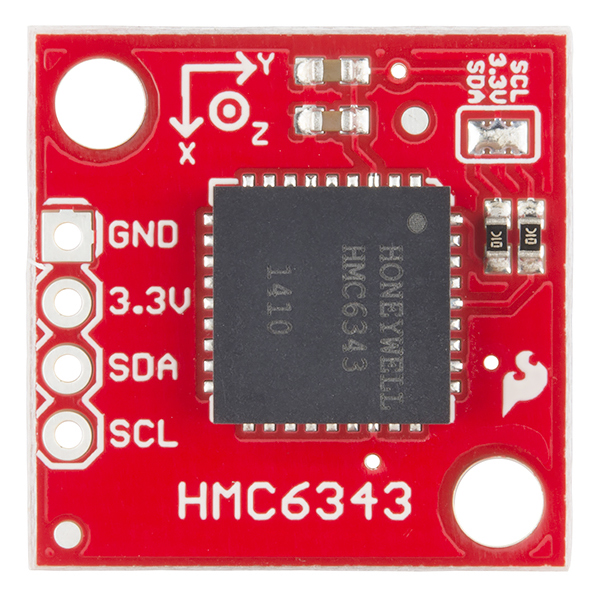
\includegraphics[width=0.6\linewidth]{./figs/IMU-HMC6343}
	
	\begin{small}
		FONTE: \cite{IMU}
	\end{small}
	\label{fig:IMU}
\end{figure}

\subsection{Circuitos eletrônicos}

\subsection{Atuadores}

O controle de atitude é feito através de atuadores que variam e muito de aplicação em aplicação. O controle é dividido em duas categorias, controle passivo e controle ativo. O controle passivo é todo aquele em que o posicionamento do satélite é feito através da tendência do mesmo em ficar em uma determinada posição. Isso significa que o satélite não pode mudar seu posicionamento, isso é definido na fase de projeto e não pode ser alterado. É usado apenas quando não há necessidade de controlar o posicionamento dele. Pode ser feito por gradiente de gravidade ou alinhamento das linhas de campo magnético. Já controle ativo é quando o posicionamento do satélite importa e precisa ser alterado. Pode ser feito através da estabilização por rotação, propulsão ou estabilização dos três eixos \cite{FrancLav}.

Para usar o método de estabilização por gradiente de inércia, o CubeSat deve ser do tipo 2U ou superior, uma vez que é necessário possuir um eixo muito mais longo que os outros. Esse eixo, que possui menor momento de inércia, ficará apontado para o centro da Terra. É um método que permite o satélite a sempre voltar para a mesma posição, mas o tempo em que isso ocorre pode variar, além dele tender a ficar oscilando em torno do eixo vertical \cite{FrancLav}.

O método de alinhamento por campo magnético é um pouco mais sofisticado, nele são colocadas bobinas, hastes magnéticas ou ímãs permanentes no satélite que geram um campo magnético próprio que tende a se orientar com o da Terra, como ilustrado na Figura \ref{fig:Mag_Field}. Pode ser utilizado sem restrições de tamanho, mas é pouco preciso, uma vez que o campo magnético da Terra é extremamente variável \cite{FrancLav}. Uma variação comum é a utilização de magnetorquers, que são basicamente hastes magnéticas que geram um campo magnético que interage com o da Terra, formando um torque e movendo o satélite. Essa já é uma forma de controle ativo mas pode interferir na medição de alguns tipos de sensores.

\begin{figure}[th]
	\caption{Alinhamento por campo magnético}
	\centering
	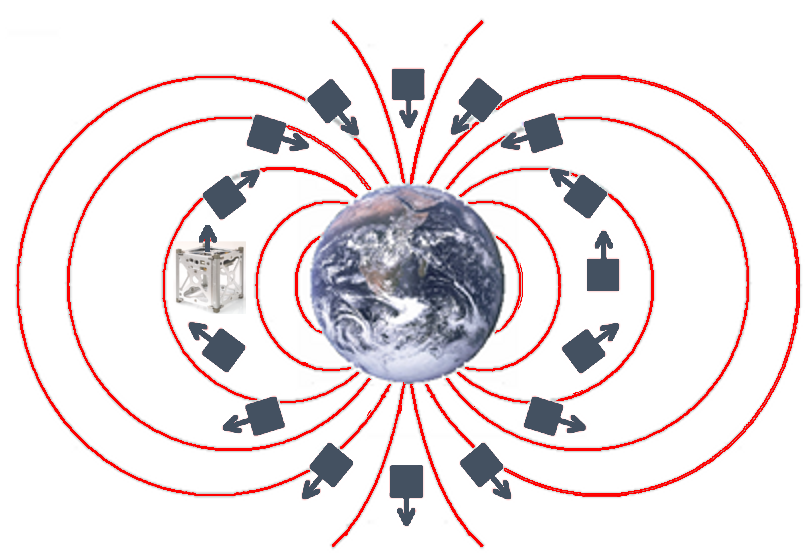
\includegraphics[width=0.8\linewidth]{./figs/Mag_Field}
	
	\begin{small}
		FONTE: \cite{FrancLav}
	\end{small}
	\label{fig:Mag_Field}
\end{figure}

O método da estabilização por rotação é uma melhoria do método passivo por alinhamento. Nele, o satélite permanece apontado para uma posição fixa e rotaciona ao redor do eixo principal. Apesar do controle não permitir mudanças bruscas no apontamento do eixo principal, que assim como o método passivo, deve ser definido durante a fase de projeto, essa rotação cria uma inércia que o torna robusto a perturbações, aumentando a precisão do apontamento \cite{FrancLav}.

O método da propulsão é muito pouco utilizado em CubeSats. Consiste em jatos de gás ou foguetes monopropulsores, que trabalham normalmente em pares, posicionados ao redor do satélite de forma que gerem um impulso inicial, provocando um torque. A vantagem dessa forma de controle é que pode ser usada também para translação do CubeSat, como ilustrado na Figura \ref{fig:Propulsion} a seguir. Porém, como ocupa muito espaço, tanto para o próprio propulsor quanto para o combustível que utiliza, é utilizado apenas em CubeSats com pelo menos 3U \cite{Luka}.

\begin{figure}[th]
	\caption{Controle através de propulsão}
	\centering
	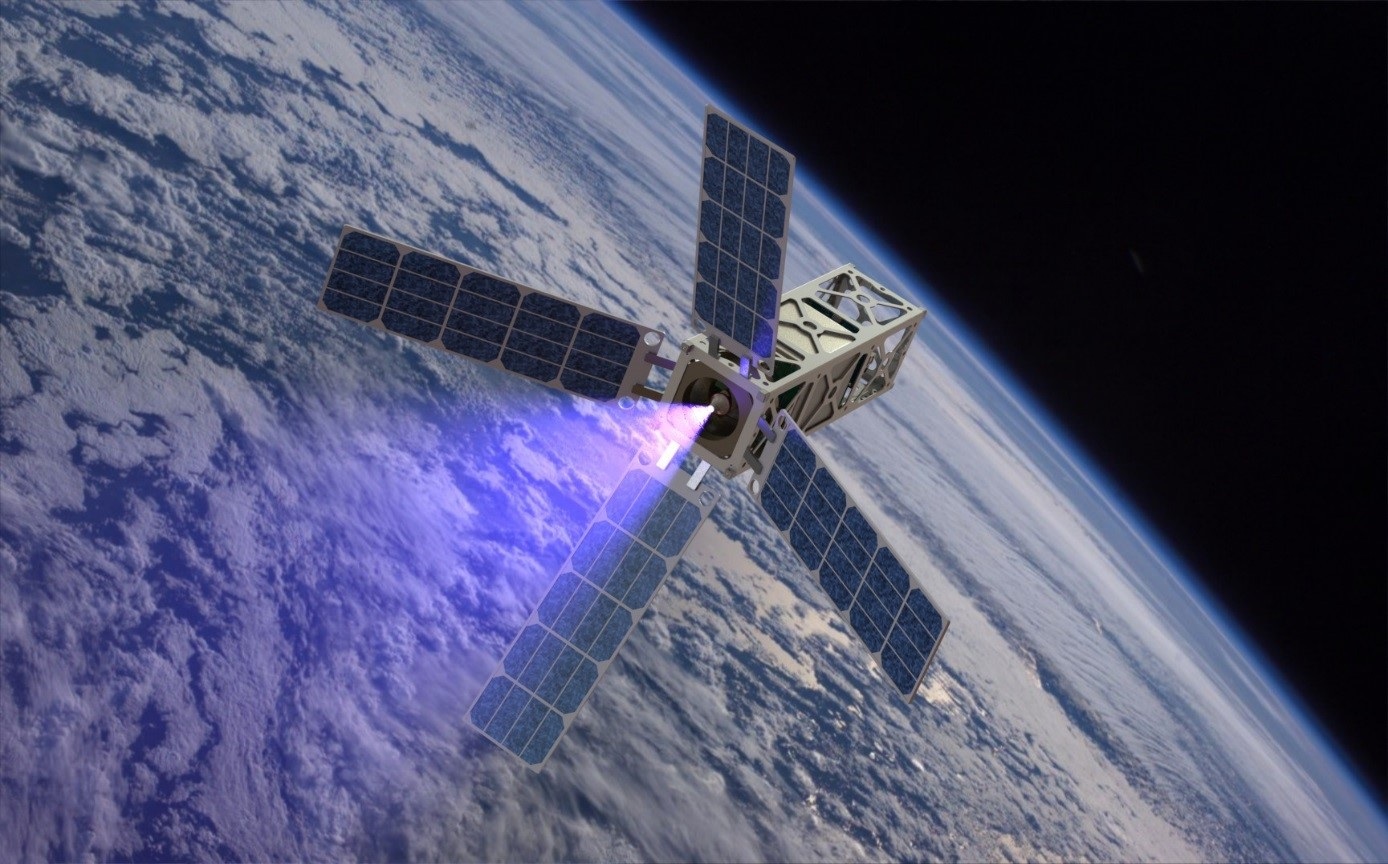
\includegraphics[width=0.8\linewidth]{./figs/Propulsion}
	
	\begin{small}
		FONTE: \cite{Prop}
	\end{small}
	\label{fig:Propulsion}
\end{figure}

O método da estabilização dos três eixos é o método mais comumente utilizado, já que é versátil e usa pouco espaço, além de ser o mais eficiente. Ele se baseia na terceira Lei de Newton, que diz: \textit{''Para toda ação, há sempre uma reação oposta e de igual intensidade''}. Isso significa que se há uma massa acelerando presa ao satélite, ela irá forçar o mesmo a girar na direção oposta. Quanto maior o valor dessa massa, mais influência ela terá sobre o sistema \cite{Ericksson}. As rodas de reação fazem o papel dessa massa ao serem fixadas ao eixo de motores (normalmente \textit{brushless}) e dispostos cada um em um eixo, possibilitando realizar manobras de rolagem (roll ou X), arfagem (pitch ou Y) e guinada (yaw ou Z).

\begin{figure}[th]
	\caption{Conjunto motor e roda de reação}
	\centering
	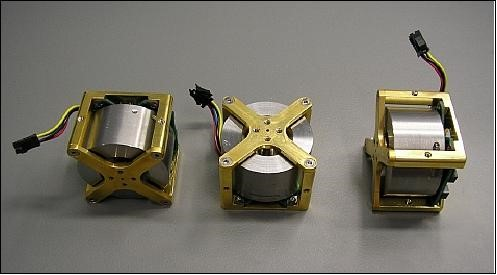
\includegraphics[width=0.7\linewidth]{./figs/Shelf_Reaction_Wheel}
	
	\begin{small}
		FONTE: \cite{SWR}
	\end{small}
	\label{fig:SRW}
\end{figure}

\newpage 

Há ainda dois tipos de controle através desse método, um com quatro e outro com três conjuntos motor-roda de reação. O modelo que utiliza quatro conjuntos possui controle mais complexo, uma vez que estes conjuntos são dispostos de forma que a somatória das rotações forma o torque desejado, como mostra a Figura \ref{fig:ERW} a seguir. Este método é amplamente utilizado pois caso um dos motores pare de funcionar, os outros três podem compensá-lo, aumentando a vida útil do satélite \cite{Ericksson}.

\begin{figure}[th]
	\caption{Modelo com quatro conjuntos motor-roda de reação e duas hastes magnéticas}
	\centering
	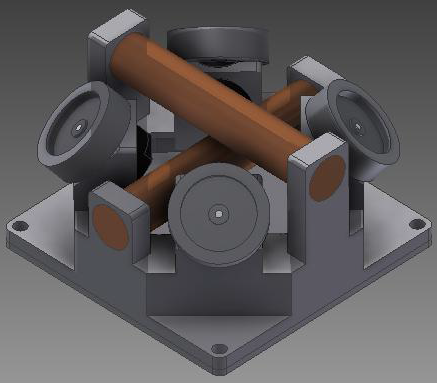
\includegraphics[width=0.7\linewidth]{./figs/Ericksson_Reaction_Wheel}
	
	\begin{small}
		FONTE: \cite{Ericksson}
	\end{small}
	\label{fig:ERW}
\end{figure}

Já o modelo de três conjuntos motor-roda de reação é mais simples, cada conjunto atua diretamente em um eixo, controlando-o diretamente, como mostrado a seguir pela Figura \ref{fig:3RW}. Sua maior desvantagem é que caso um dos motores pare de funcionar, o movimento do satélite no eixo correspondente também cessa. Esse é o método adotado e explorado nesse trabalho.

\begin{figure}[th]
	\caption{Modelo com três conjuntos motor-roda de reação}
	\centering
	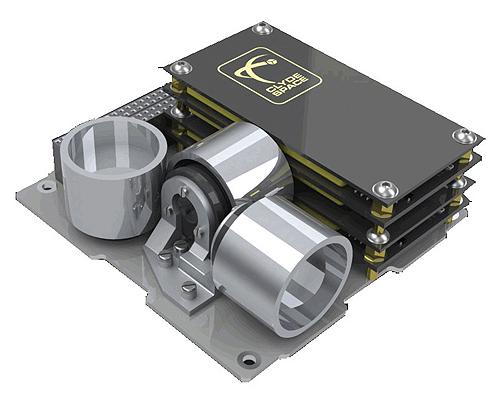
\includegraphics[width=0.7\linewidth]{./figs/3RW}
	
	\begin{small}
		FONTE: \cite{3RW}
	\end{small}
	\label{fig:3RW}
\end{figure}

Para integração do motor adotado com a roda de ação, foi criado um conjunto padrão que consiste em um suporte para o motor, o motor e a roda de reação. Foi utilizado um desses conjuntos em cada um dos eixos correspondentes ao \textit{roll}, \textit{pitch} e \textit{yaw} como mostrado na Figura \ref{fig:MotSet} a seguir.

\begin{figure}[th]
	\caption{Conjunto para acoplamento do motor ao CubeSat}
	\centering
	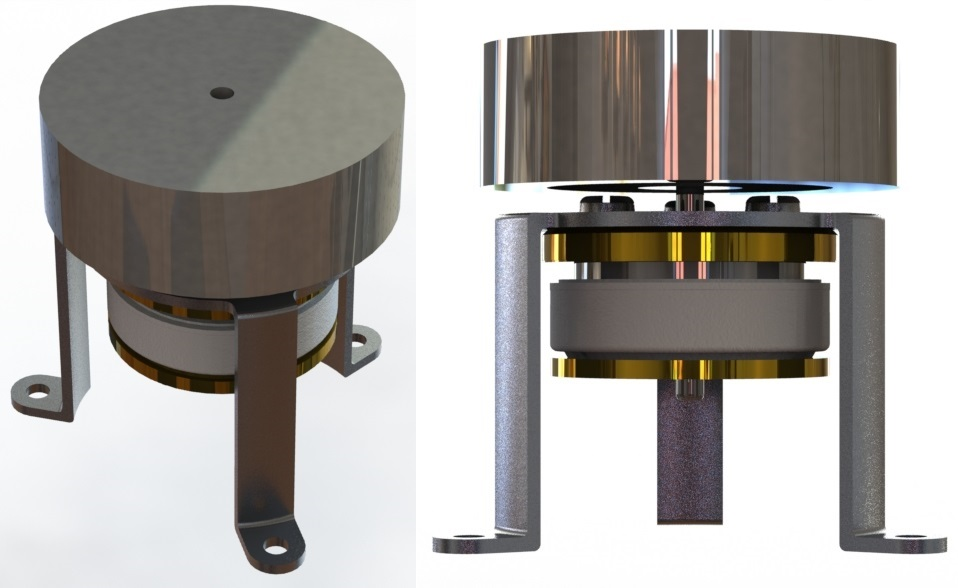
\includegraphics[width=0.69\linewidth]{./figs/Motor_Set}
	
	\begin{small}
		FONTE: Arquivo dos autores
	\end{small}
	\label{fig:MotSet}
\end{figure}

\subsubsection{Motores}

Para escolha do motor, foi levado em considerado principalmente três fatores: tipo, tamanho e potência \cite{Ericksson}.

Costumeiramente, CubeSats utilizam motores de corrente contínua sem escovas (\textit{brushless direct current motor} – BLDC). A NASA recomenda o uso de motores desse tipo para aplicações aero-espaciais \cite{NASABLDC}. A tabela \ref{tab:VnteDesv} a seguir mostra um comparativo das principais vantagens do uso de um motor \textit{Brushless} na área aeroespacial.

\begin{table}[h]
	\caption{Vantagens e desvantagens de um motor \textit{Brushless}}
		\centering
	\begin{tabular}{|c|c|}
		\hline 
		\textbf{Vantagens} & \textbf{Desvantagens} \\ 
		\hline 
		Alta velocidade (até 100000 RPM) & Circuitos mais caros \\ 
		\hline 
		Alto torque a altas velocidades & Maior complexidade do driver do motor \\ 
		\hline 
		Aproximadamente o dobro de torque & \\
		 de saída quando comparado a motores & \\
		  com escova do mesmo tamanho &  \\ 
		\hline 
		Enrolamentos no estator ao invés & \\
		 do rotor melhoram a dissipação & \\
		  de calor & \\ 
		\hline 
		Sem escovas, então os motores & \\
		 duram enquanto durarem os & \\
		  rolamentos & \\ 
		\hline 
		Alta eficiência & \\ 
		\hline 
		Bom desempenho no vácuo & \\ 
		\hline
	\end{tabular}
	
	\begin{small}
	FONTE: \cite{Ericksson}
	\end{small}
	\label{tab:VnteDesv}
\end{table}

O tamanho do motor também é um fator limitante pois o espaço dentro de um CubeSat é extremamente limitado. Quanto menor o tamanho dos motores, mais fácil de acomodá-los e mais espaço sobra para utilizar com outros fatores, como a bateria no caso de um CubeSat de 1 U ou para acomodar outras pesquisas que o CubeSat possa estar levando \cite{Martins}.

\begin{figure}[th]
	\caption{Motor Maxon 351100, a moeda serve para referência quanto às dimensões}
	\centering
	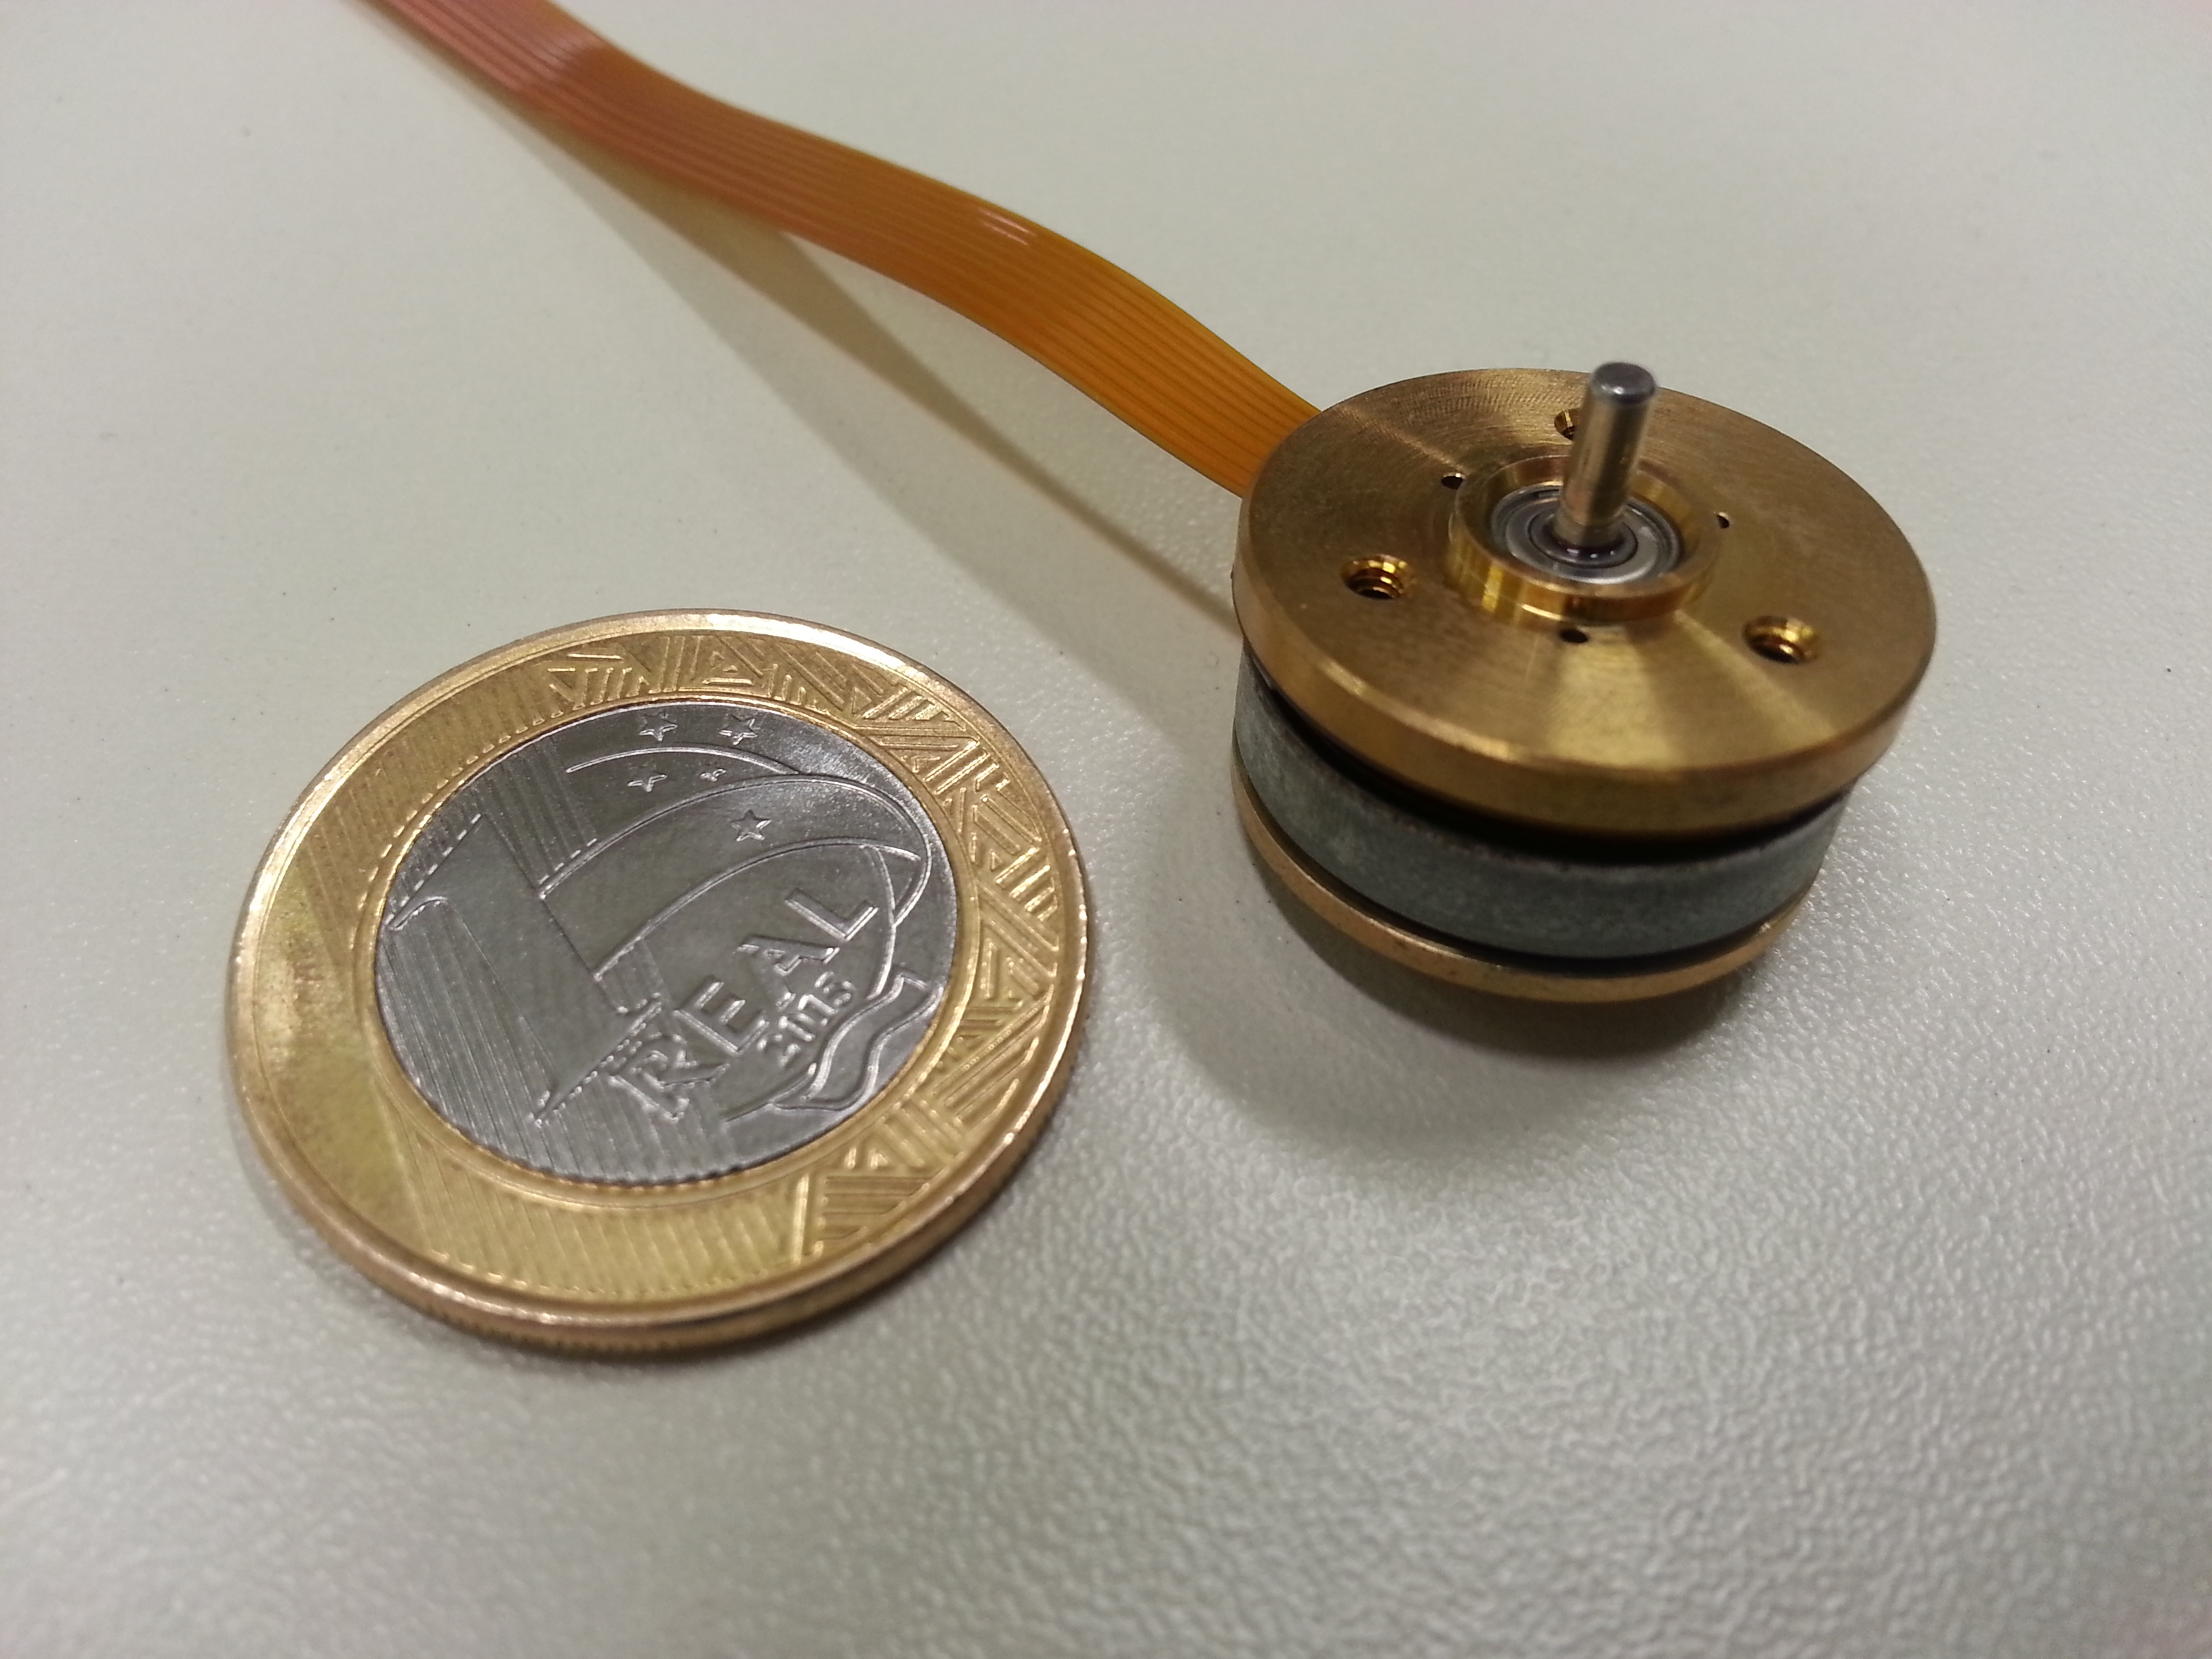
\includegraphics[width=0.8\linewidth]{./figs/Maxon_351100}
	
	\begin{small}
		FONTE: Arquivo dos autores
	\end{small}
	\label{fig:Maxon}
\end{figure}

\subsubsection{Rodas de reação}

A roda de reação é basicamente um disco rotativo com muita massa (em relação ao resto do sistema). Quanto maior a massa e a geometria dela, maior a inércia I (kgm$^2$), como demonstrado na equação \ref{eq:Inercia}, onde m (kg) é a massa e r (m) é o raio da roda. A inércia cresce proporcionalmente ao quadrado o raio da roda.

\begin{equation}
I= \frac{m}{2} \times r^2
\label{eq:Inercia}
\end{equation}

A relação entre a massa da roda de reação com a massa do satélite influencia diretamente na forma como o controle é feito. Como dito anteriormente, quanto maior a massa da roda de reação, e consequentemente a inércia dele, melhor para o controle. Porém, dada a limitação de espaço hábil dentro do CubeSat, não é possível projetar uma roda de reação com grande raio. Para compensar, a roda utilizada deverá ter uma massa mais elevada, e a forma de conseguir isso com dimensões limitadas é utilizando materiais mais densos. Nesse caso, a roda foi projetada considerando aço, como mostrado a seguir na Figura \ref{fig:RW}.

\begin{figure}[th]
	\caption{Roda de reação}
	\centering
	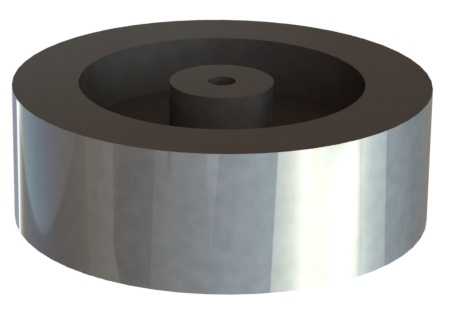
\includegraphics[width=0.5\linewidth]{./figs/Reaction_Wheel}
	
	\begin{small}
		FONTE: Arquivo dos autores
	\end{small}
	\label{fig:RW}
\end{figure}

Por causa da forma como o motor é preso no suporte, foi necessário um pequeno rasgo na roda de reação com o objetivo de evitar que as cabeças dos parafusos interferissem na roda de reação.

Apesar da roda projetada ser cilíndrica, ela não possui a mesma seção para toda sua extensão, e a equação \ref{eq:Inercia} se aplica a corpos cilíndricos homogêneos. Para o cálculo correto da inercia, aplica-se a equação \ref{eq:Inercia} para cada seção e então se aplica a equação \ref{eq:Inetot}.

\begin{equation}
I_{total} = \sum\nolimits I_{1} + I_{2} + I_{3}
\label{eq:Inetot}
\end{equation}

As rodas foram usinadas em em aço 1020, em um torno CNC. O peso delas ficou igual a  kg. A Inércia, portante, ficou igual a  kgm$^2$.

\subsubsection{Suporte do motor}

Para suportar o motor, foi desenvolvido um protótipo genérico obedecendo as furações dos motores e o espaço para o eixo para a fixação dos mesmos ao suporte e dele à placa de circuito eletrônico do CubeSat. Esse suporte foi feito com altura de 10 mm da superfície inferior do motor até a placa de circuito eletrônico para que não atrapalhasse o posicionamento dos componentes, como mostrado na Figura \ref{fig:MS} a seguir. Para atender aos requisitos de peso, o suporte foi projetado em alumínio.

\begin{figure}[th]
	\caption{Suporte do motor}
	\centering
	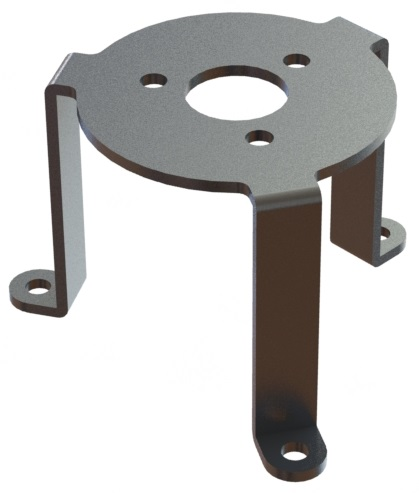
\includegraphics[width=0.5\linewidth]{./figs/Motor_Sup}
	
	\begin{small}
		FONTE: Arquivo dos autores
	\end{small}
	\label{fig:MS}
\end{figure}

Os suportes foram fabricados com chapas de alumínio de 1 mm de espessura através de uma máquina de corte a laser e então dobrados. O peso ficou igual a  kg.

\subsection{Estrutura mecânica}

A estrutura mecânica do CubeSat foi projetada seguindo os padrões indicados pela Cal Poly \cite{CalPoly}. O projeto foi feito pelo Núcleo de Sistemas Eletrônicos Embarcados (NSEE) da Mauá, que é responsável pelo desenvolvimento do CubeSat Mauá, sendo de nossa responsabilidade apenas o sistema de controle de atitude do satélite. O modelo básico no qual o trabalho se desenvolverá é mostrado a seguir apenas com a estrutura mecânica em si a mostra na Figura \ref{fig:Frame}.

\begin{figure}[th]
	\caption{Estrutura do CubeSat}
	\centering
	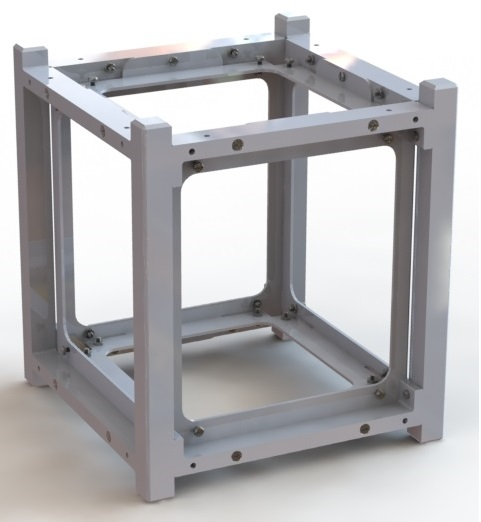
\includegraphics[width=0.7\linewidth]{./figs/Frame}
	
	\begin{small}
		FONTE: Arquivo dos autores
	\end{small}
	\label{fig:Frame}
\end{figure}

\newpage

\section[Métodos]{Métodos}



\subsection{Modelagem}



\subsubsection{Rodas de reação}

Ao aplicar uma tensão V (V) em um motor elétrico, uma corrente i (A) passará pelos enrolamentos dele e será convertida em um torque mecânico T$_{m}$ (kgm$^{2}$/s$^{2}$). No motor, há uma resistência R ($\Omega$) devido aos enrolamentos das bobinas. É nessas bobinas que a corrente induz um campo magnético que força o eixo do motor a girar. A resistência interna do motor causa uma queda de tensão V$_{emf}$ (V), que é mostrada na equação \ref{eq:Tens}.

\begin{equation}
V = i \times R + V_{emf}
\label{eq:Tens}
\end{equation}

A relação entre a corrente no motor e o torque T$_{m}$ é descrita na equação \ref{eq:Torq}, com a constante de torque k$_{T}$ (Nm/A).

\begin{equation}
T_{m} = k_{T} \times i
\label{eq:Torq}
\end{equation}

A queda de tensão no motor resulta em uma perda de potência. Essa perda, P$_{T}$, costuma ser pequena caso o motor esteja em boas condições e sem nenhum defeito. A equação \ref{eq:PowerLoss} mostra como obter esse valor, onde $\eta$ é a eficiência do motor e $\omega_{w}$ é a velocidade angular.

\begin{equation}
P_{T} = V_{emf} \times i = \eta \times T_{m} \times \omega_{w} \approx T_{m} \times \omega_{w} = k_{T} \times i \times \omega_{w}
\label{eq:PowerLoss}
\end{equation}

O V$_{emf}$ pode ser descrito como na equação \ref{eq:Vemf}, onde k$_{T}$ e k$_{E}$ (Vs/rad) são o mesmo para um motor com 100\% de eficiência.

\begin{equation}
V_{emf} = k_{T} \times \omega_{w} \equiv k_{E} \times \omega_{w}
\label{eq:Vemf}
\end{equation}

Aproveitando a equação de dinâmica da roda de reação, temos a equação \ref{eq:Tm}, onde I$_{w}$ é o total de inércia do motor junto da roda de reação, B é o atrito viscoso e $\dot{\omega}_{w}$ é a aceleração angular.

\begin{equation}
T_{m} = I_{w} \times \dot{\omega}_{w} + B \times \omega_{w}
\label{eq:Tm}
\end{equation}

A equação \ref{eq:Tens} é reescrita como,

\begin{equation}
i = \frac{V - V_{emf}}{R}
\label{eq:I}
\end{equation}

Ao substituir i na equação \ref{eq:Torq}, com a equação \ref{eq:I} e substituindo o V$_{emf}$ pela equação \ref{eq:Vemf}, obtemos uma expressão igual à equação \ref{eq:Tm}, mostrado a seguir.

\begin{equation}
T_{m} = k_{T} \times i = k_{T} \times \frac{V - V_{emf}}{R} = k_{T} \times \frac{ V - k_{E} \times \omega_{w} }{R} = I_{w} \times \dot{\omega}_{w} + B \times \omega_{w}
\label{eq:Subst}
\end{equation}

A expressão \ref{eq:Subst} é reescrita como,

\begin{equation}
\frac{k_{T}}{R} \times V = I_{w} \times \dot{\omega}_{w} + \frac{(R \times B + k_{E} \times k_{T}) \times \omega_{w} }{R}
\label{eq:ReWrite}
\end{equation}

Isola-se então o $\omega_{w}$ da equação \ref{eq:ReWrite}, obtendo.

\begin{equation}
\left( \frac{k_{T}}{R \times B + k_{E} \times k_{T}} \right) \times V = \left( \frac{R \times I_{w}}{R \times B + k_{E} \times k_{T}} \right) \times \dot{\omega}_{w} + \omega_{w}
\label{eq:ReW}
\end{equation}

Da equação \ref{eq:ReW}, é possível observar que os valores em parênteses são constantes. Portanto, a equação pode ser reescrita da seguinte forma,

\begin{equation}
C \times V = \tau \times \dot{\omega}_{w} + \omega_{w}
\label{eq:RWDM}
\end{equation}

Onde C e $\tau$ são constantes. Portanto, a equação \ref{eq:RWDM} é o modelo dinâmico do conjunto roda de reação e motor \cite{Ericksson}.

\subsection{Controle}



% ----------------------------------------------------------
% PROTÓTIPO 
% ----------------------------------------------------------
\chapter[Protótipo]{Protótipo}



\section{Rodas de reação}

Os protótipos das rodas de reação foram feitos em um torno CNC (, )pela empresa Rudloff, através de uma parceria entre a Mauá e a empresa. A seguir, na Figura , uma imagem de como ficaram.

%\begin{figure}[th]
%	\caption{Modelo das rodas de reação}
%	\centering
%	\includegraphics[width=0.7\linewidth]{./figs/}
%	
%	\begin{small}
%		FONTE: Arquivo dos autores
%	\end{small}
%	\label{fig:ProtoRW}
%\end{figure}

\section{Suporte do motor}

Para uma pré validação do projeto do suporte do motor, foi feito um modelo impresso em uma impressora 3D (Cliever, Porto Alegre, RS), como mostrado a seguir na Figura . Esse modelo foi usado para garantir o batimento dos furos do suporte com os do motor.

%\begin{figure}[th]
%	\caption{Protótipo em resina do suporte do motor}
%	\centering
%	\includegraphics[width=0.7\linewidth]{./figs/}
%	
%	\begin{small}
%		FONTE: Arquivo dos autores
%	\end{small}
%	\label{fig:ProtoMSP}
%\end{figure}

Uma vez validado, foi mandado fazer um modelo em metal, através do corte por máquina de corte laser (, ) e dobra, através de uma dobradeira (, ). Esse modelo é mostrado a seguir, na Figura .

%\begin{figure}[th]
%	\caption{Modelo em metal do suporte do motor}
%	\centering
%	\includegraphics[width=0.7\linewidth]{./figs/}
%	
%	\begin{small}
%		FONTE: Arquivo dos autores
%	\end{small}
%	\label{fig:ProtoMS}
%\end{figure}

\section{Estrutura mecânica}

Um primeiro protótipo da estrutura mecânica foi fabricado na oficina mecânica da Mauá para que pudessem ser feitos os primeiros testes de encaixe, tanto da própria estrutura quanto das placas de circuito eletrônico. A seguir, a estrutura montada na Figura \ref{fig:ProtooneF}.

\begin{figure}[ht]
	\caption{Primeiro protótipo do CubeSat fechado}
	\centering
	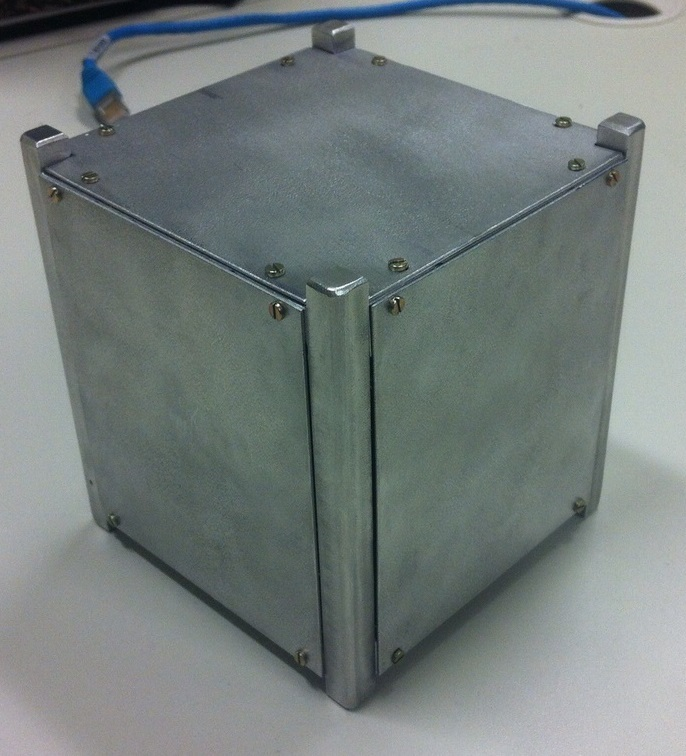
\includegraphics[width=0.7\linewidth]{./figs/PrototypeOne_Full}
	
	\begin{small}
		FONTE: Arquivo dos autores
	\end{small}
	\label{fig:ProtooneF}
\end{figure}

\newpage

Com duas chapas de fechamento removidas a seguir, na Figura \ref{fig:Protoone}.

\begin{figure}[ht]
	\caption{Primeiro protótipo do CubeSat com duas chapas de fechamento removidas}
	\centering
	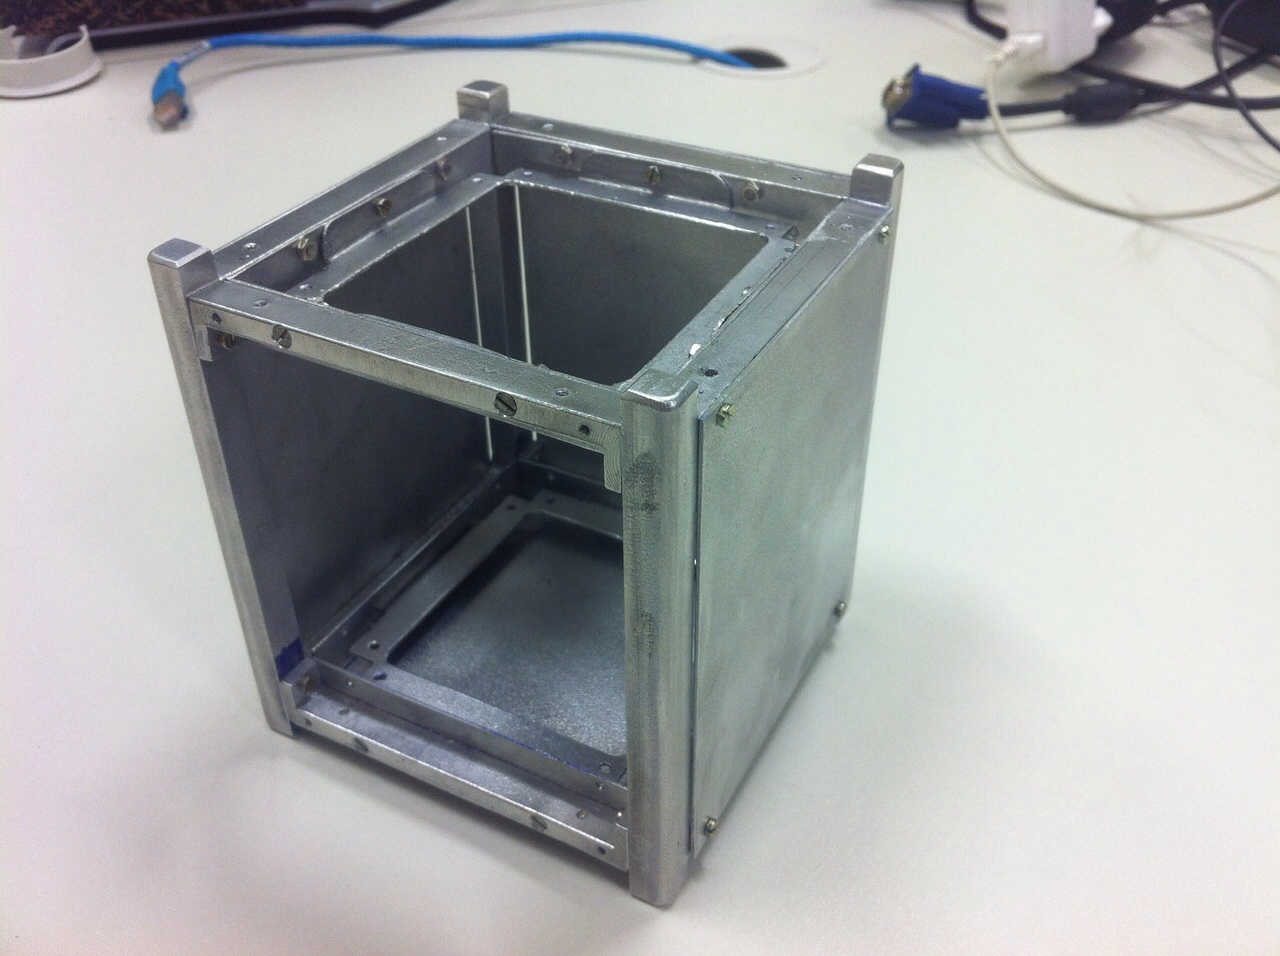
\includegraphics[width=0.7\linewidth]{./figs/PrototypeOne}
	
	\begin{small}
		FONTE: Arquivo dos autores
	\end{small}
	\label{fig:Protoone}
\end{figure}

Posteriormente, foram feitos ajustes nos desenhos em CAD e uma nova versão foi feita. As partes de chapas foram feitas em máquinas de corte laser e dobradas, caso necessário, por uma empresa especializada. As outras partes foram feitas em um centro de usinagem (, ) no laboratório de usinagem da Mauá. O modelo finalizado sem as chapas de fechamento a seguir, na Figura .

%\begin{figure}[th]
%	\caption{Modelo em metal do suporte do motor}
%	\centering
%	\includegraphics[width=0.7\linewidth]{./figs/}
%	
%	\begin{small}
%		FONTE: Arquivo dos autores
%	\end{small}
%	\label{fig:ProtoTwo}
%\end{figure}

% ----------------------------------------------------------
% RESULTADOS E DISCUSSÕES
% ----------------------------------------------------------
\chapter[Resultados e discussões]{Resultados e discussões}

% ----------------------------------------------------------
% CONCLUSÕES
% ----------------------------------------------------------
\chapter[Conclusões]{Conclusões}

% ----------------------------------------------------------
% REFERÊNCIAS BIBLIOGRÁFICAS
% ----------------------------------------------------------
\bibliography{TCC_Sist_Controle_Atitude}

% ----------------------------------------------------------
% Apêndices
% ----------------------------------------------------------
% Inicia os apêndices
% ---
\begin{apendicesenv}
% Imprime uma página indicando o início dos apêndices
\partapendices
% ---
\chapter{Desenho do suporte do motor}



\chapter{Desenho da roda de reação}



\end{apendicesenv}

% ----------------------------------------------------------
% Anexos
% ----------------------------------------------------------
% Inicia os anexos
% ---
\begin{anexosenv}
% Imprime uma página indicando o início dos anexos
\partanexos
% ---
\chapter{Página do catálogo do motor brushless 351100 da Maxon}

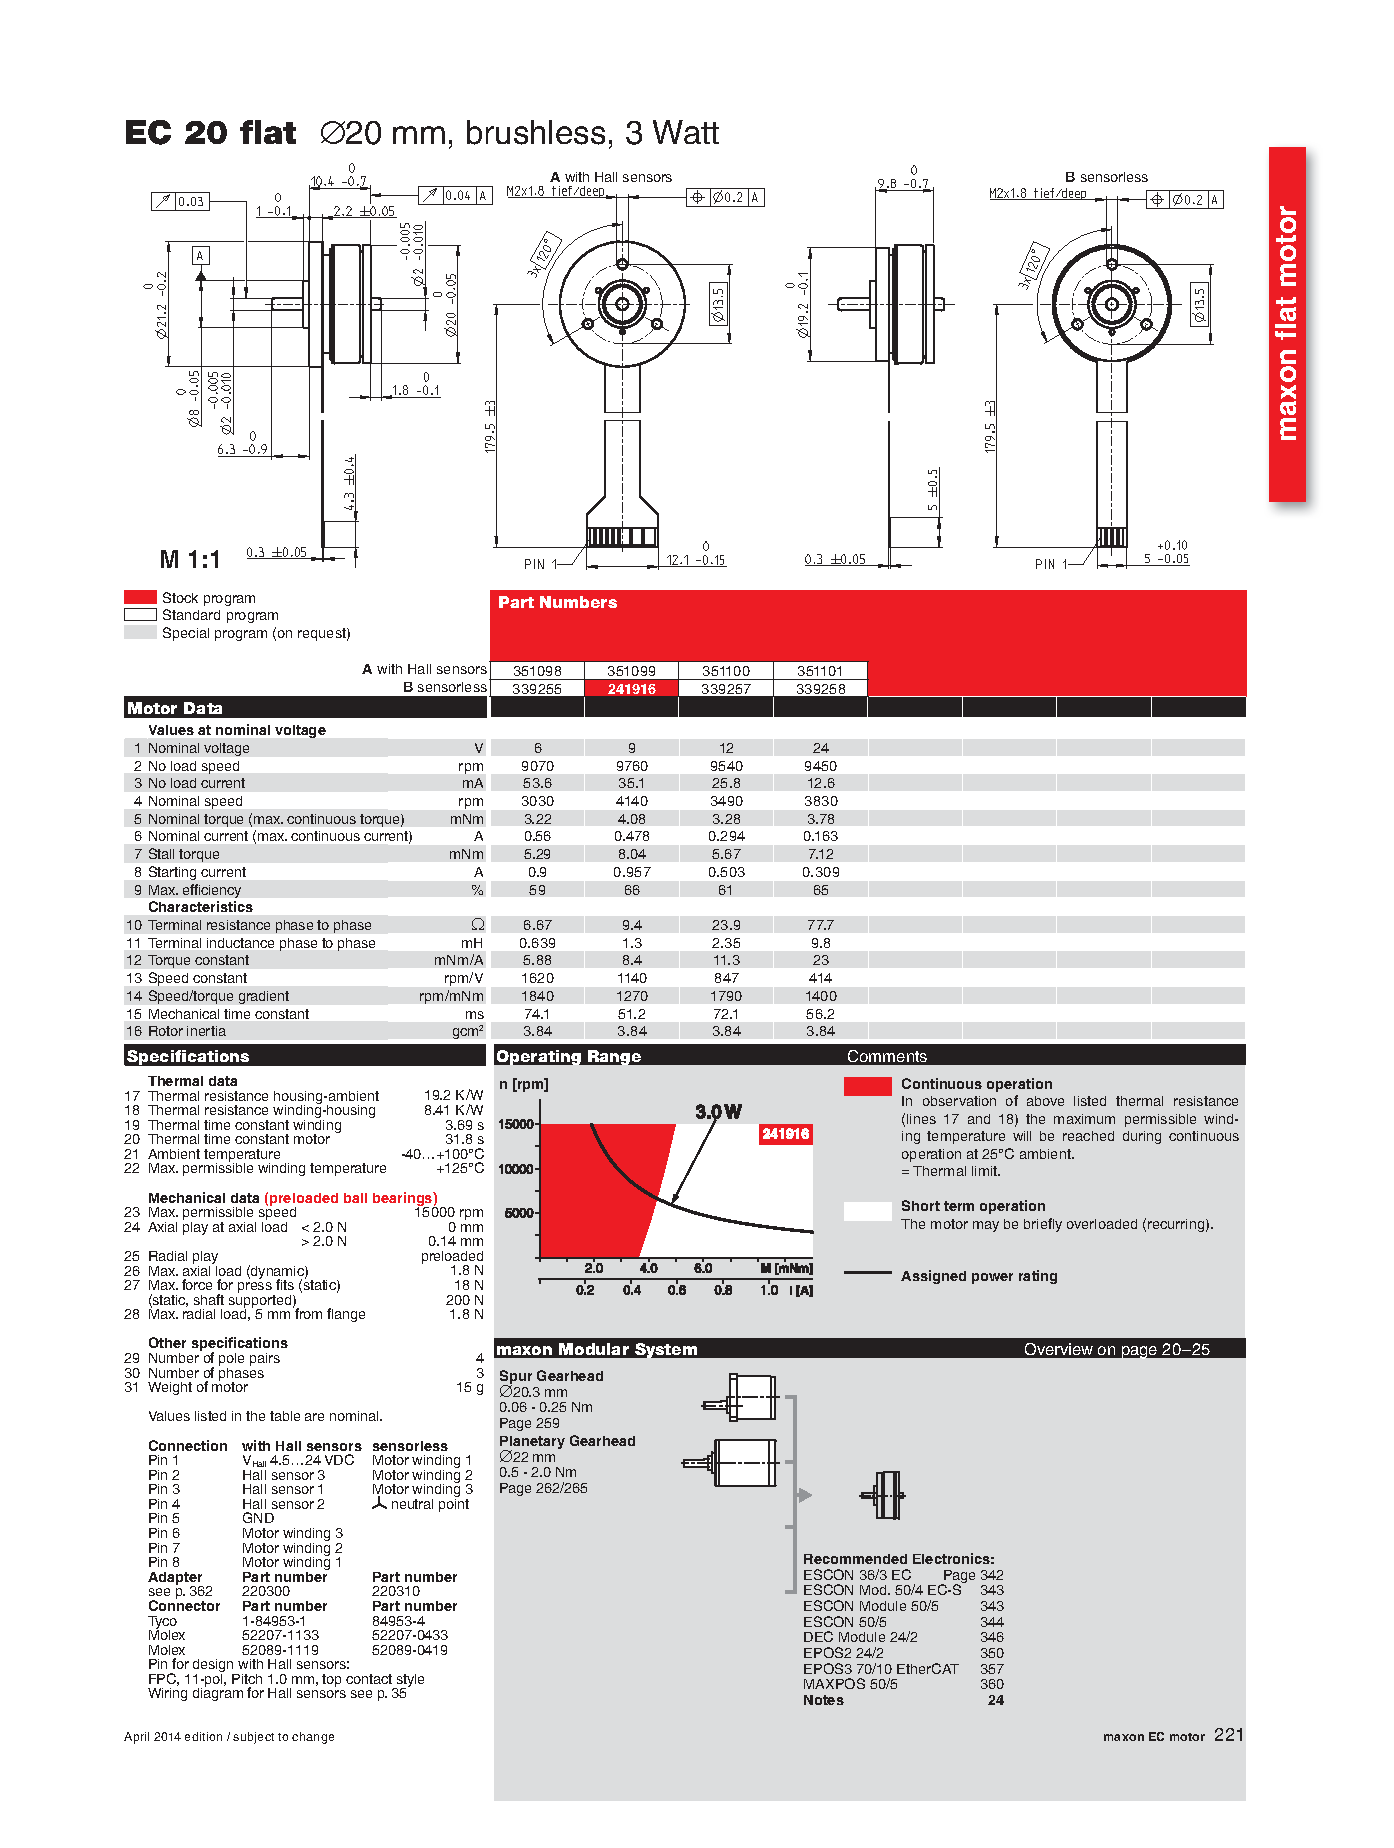
\includepdf[pages=-]{./pdfs/351100.pdf}

\end{anexosenv}

\end{document}